\section{lib/efreet\_\-xml.c File Reference}
\label{efreet__xml_8c}\index{lib/efreet\_\-xml.c@{lib/efreet\_\-xml.c}}


{\tt \#include \char`\"{}Efreet.h\char`\"{}}\par
{\tt \#include \char`\"{}efreet\_\-private.h\char`\"{}}\par


Include dependency graph for efreet\_\-xml.c:\nopagebreak
\begin{figure}[H]
\begin{center}
\leavevmode
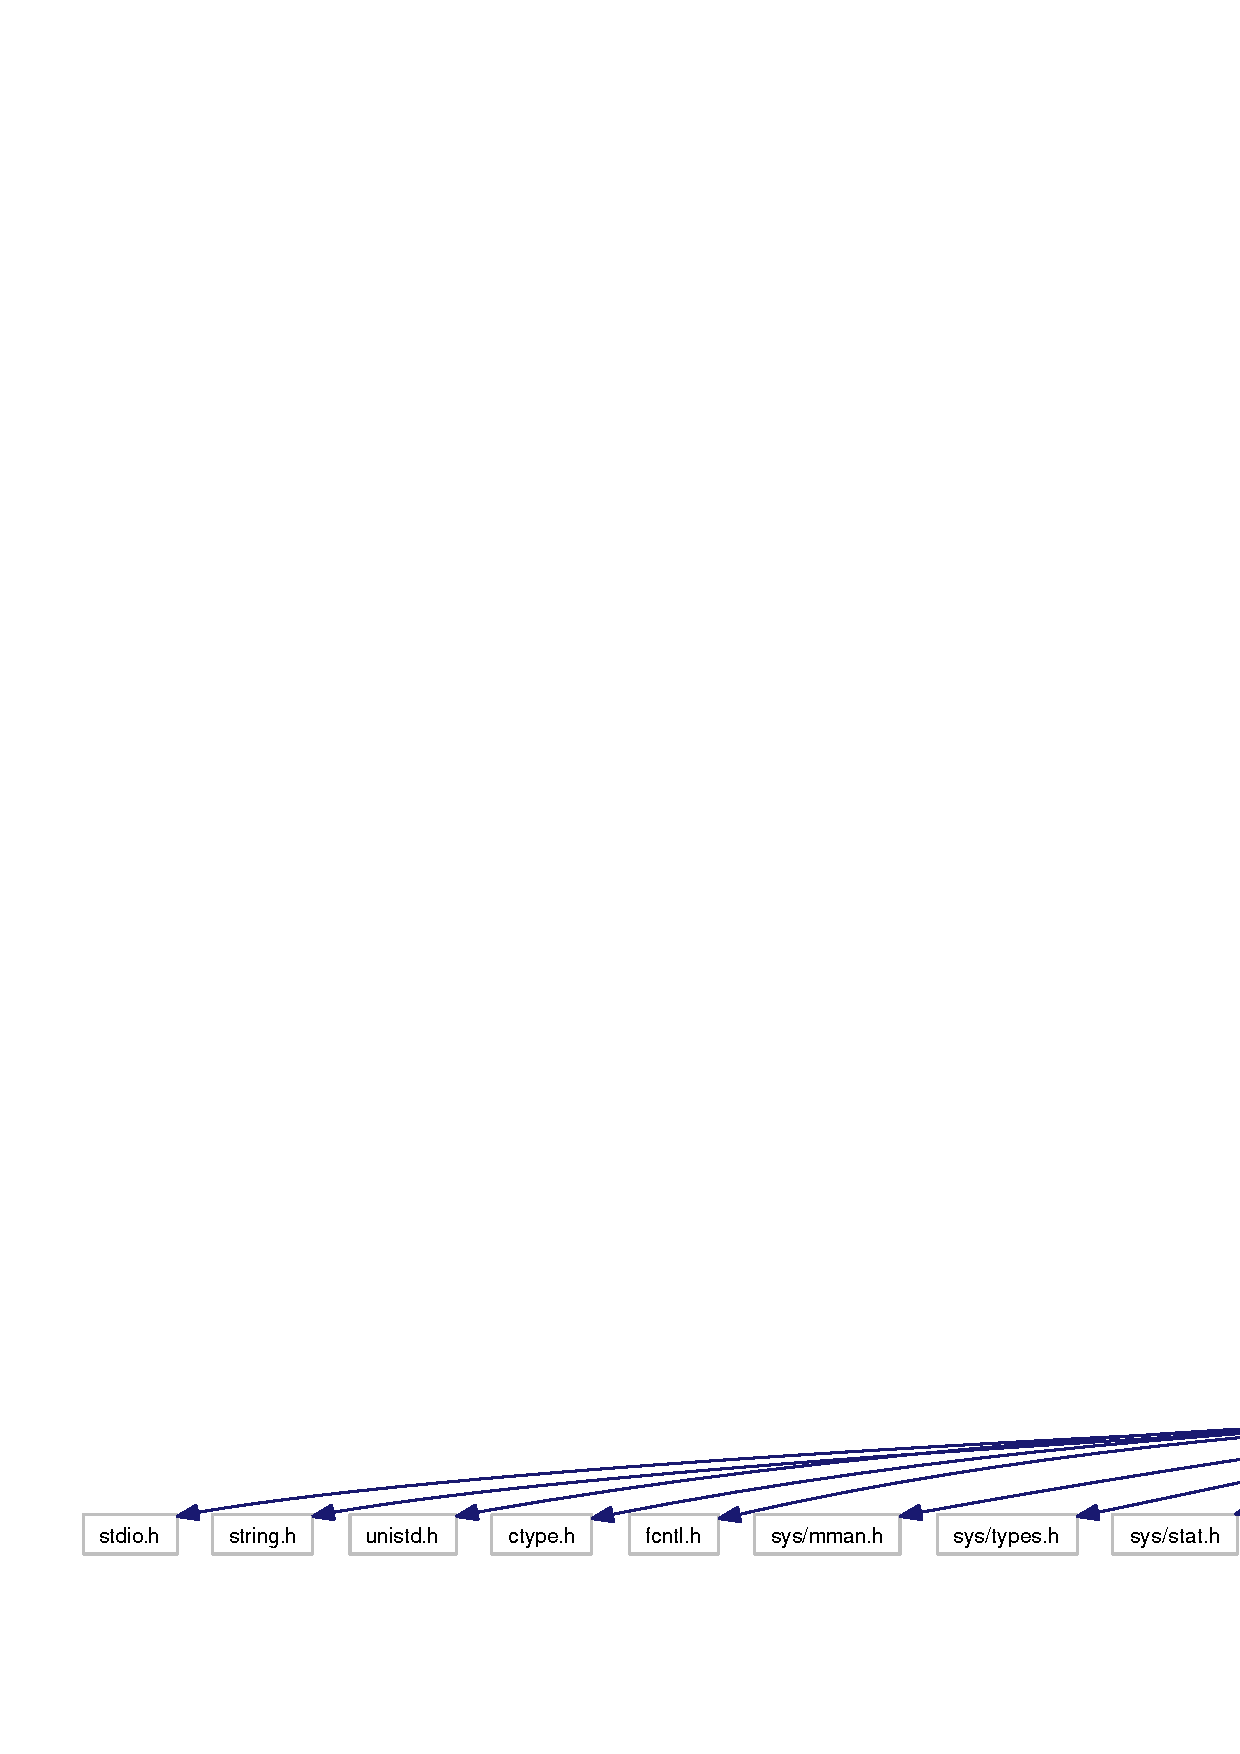
\includegraphics[width=420pt]{efreet__xml_8c__incl}
\end{center}
\end{figure}
\subsection*{Functions}
\begin{CompactItemize}
\item 
const char $\ast$ {\bf efreet\_\-xml\_\-attribute\_\-get} ({\bf Efreet\_\-Xml} $\ast$xml, const char $\ast$key)
\begin{CompactList}\small\item\em Retrieves the value for the given attribute key. \item\end{CompactList}\item 
void {\bf efreet\_\-xml\_\-del} ({\bf Efreet\_\-Xml} $\ast$xml)
\item 
int {\bf efreet\_\-xml\_\-init} (void)
\item 
{\bf Efreet\_\-Xml} $\ast$ {\bf efreet\_\-xml\_\-new} (const char $\ast$file)
\item 
int {\bf efreet\_\-xml\_\-shutdown} (void)
\end{CompactItemize}


\subsection{Function Documentation}
\index{efreet\_\-xml.c@{efreet\_\-xml.c}!efreet\_\-xml\_\-attribute\_\-get@{efreet\_\-xml\_\-attribute\_\-get}}
\index{efreet\_\-xml\_\-attribute\_\-get@{efreet\_\-xml\_\-attribute\_\-get}!efreet_xml.c@{efreet\_\-xml.c}}
\subsubsection[efreet\_\-xml\_\-attribute\_\-get]{\setlength{\rightskip}{0pt plus 5cm}const char$\ast$ efreet\_\-xml\_\-attribute\_\-get ({\bf Efreet\_\-Xml} $\ast$ {\em xml}, \/  const char $\ast$ {\em key})}\label{efreet__xml_8c_bb8a77ca97f883d4b60c14e47099272e}


Retrieves the value for the given attribute key. 

\begin{Desc}
\item[Parameters:]
\begin{description}
\item[{\em xml,:}]The xml struct to work with \item[{\em key,:}]The attribute key to look for \end{description}
\end{Desc}
\begin{Desc}
\item[Returns:]Returns the value for the given key, or NULL if none found \end{Desc}


References Efreet\_\-Xml::attributes.\index{efreet\_\-xml.c@{efreet\_\-xml.c}!efreet\_\-xml\_\-del@{efreet\_\-xml\_\-del}}
\index{efreet\_\-xml\_\-del@{efreet\_\-xml\_\-del}!efreet_xml.c@{efreet\_\-xml.c}}
\subsubsection[efreet\_\-xml\_\-del]{\setlength{\rightskip}{0pt plus 5cm}void efreet\_\-xml\_\-del ({\bf Efreet\_\-Xml} $\ast$ {\em xml})}\label{efreet__xml_8c_43503b3ca04624a604f71e023dbc1fb8}




References Efreet\_\-Xml::attributes, Efreet\_\-Xml::children, FREE, IF\_\-FREE, Efreet\_\-Xml::tag, and Efreet\_\-Xml::text.

Referenced by efreet\_\-menu\_\-parse(), and efreet\_\-xml\_\-new().\index{efreet\_\-xml.c@{efreet\_\-xml.c}!efreet\_\-xml\_\-init@{efreet\_\-xml\_\-init}}
\index{efreet\_\-xml\_\-init@{efreet\_\-xml\_\-init}!efreet_xml.c@{efreet\_\-xml.c}}
\subsubsection[efreet\_\-xml\_\-init]{\setlength{\rightskip}{0pt plus 5cm}int efreet\_\-xml\_\-init (void)}\label{efreet__xml_8c_7a2ad4fd7dfefb664c99f198d880d606}




Referenced by efreet\_\-init(), and efreet\_\-menu\_\-init().\index{efreet\_\-xml.c@{efreet\_\-xml.c}!efreet\_\-xml\_\-new@{efreet\_\-xml\_\-new}}
\index{efreet\_\-xml\_\-new@{efreet\_\-xml\_\-new}!efreet_xml.c@{efreet\_\-xml.c}}
\subsubsection[efreet\_\-xml\_\-new]{\setlength{\rightskip}{0pt plus 5cm}{\bf Efreet\_\-Xml}$\ast$ efreet\_\-xml\_\-new (const char $\ast$ {\em file})}\label{efreet__xml_8c_4d2285311849adcc65e6988fd99aa697}




References efreet\_\-xml\_\-del().

Referenced by efreet\_\-menu\_\-parse().\index{efreet\_\-xml.c@{efreet\_\-xml.c}!efreet\_\-xml\_\-shutdown@{efreet\_\-xml\_\-shutdown}}
\index{efreet\_\-xml\_\-shutdown@{efreet\_\-xml\_\-shutdown}!efreet_xml.c@{efreet\_\-xml.c}}
\subsubsection[efreet\_\-xml\_\-shutdown]{\setlength{\rightskip}{0pt plus 5cm}int efreet\_\-xml\_\-shutdown (void)}\label{efreet__xml_8c_b23f8e3a7d790c153a0612d54967e6a3}




Referenced by efreet\_\-menu\_\-shutdown(), and efreet\_\-shutdown().